\documentclass[12pt,a4paper]{ctexart}
\usepackage[margin=2.2cm]{geometry}
\usepackage{graphicx,booktabs,amsmath,float,hyperref,xcolor,listings}
\lstset{language=Verilog,basicstyle=\ttfamily\footnotesize,keywordstyle=\color{blue!70!black},commentstyle=\color{green!40!black},stringstyle=\color{orange!60!black},showstringspaces=false,breaklines=true,columns=fullflexible,keepspaces=true,frame=single,tabsize=4}
\setlength{\emergencystretch}{2em}
\newcommand{\reporttitle}{计算机组成与系统结构专题实验\\实验三：算术逻辑单元设计}
\newcommand{\authname}{李祥熙}
\newcommand{\authid}{2234412799}
\newcommand{\class}{计算机2301}
\title{\reporttitle}
\author{姓名：\authname\quad 班级：\class\\学号：\authid}
\date{2026年11月16日}
\begin{document}
\maketitle
\tableofcontents
\newpage
\section{实验目的}
\begin{itemize}
\item 掌握一位全加器的真值表和逻辑表达式，通过结构化连接构成多位加法器。
\item 实现4位、16位和32位加法器，并实现选做的4位先行进位加法器。
\item 设计具有八种功能的32位ALU，正确产生零、进位、溢出、符号和奇偶标志。
\item 比较行为描述、多路选择与片选控制共享总线的实现方式，观察使能无效时的高阻输出。
\item 使用自检查测试平台验证运算结果、标志位和不同实现之间的一致性。
\end{itemize}
\section{实验过程}
\subsection{实验环境}
实验使用Windows系统、AMD Vivado 2026.1及其XSim仿真器，语言为Verilog，工程器件为\texttt{xc7a35tcsg324-1}。仿真时间单位为1 ns，精度为1 ps。本实验的加法器和ALU均为组合逻辑，不使用时钟。测试平台改变输入后等待10 ns，再检查结果，并记录波形。这一间隔用于分隔激励和等待组合逻辑收敛，不代表电路实际传播延迟。

\subsection{实现和验证流程}
首先按照一位全加器真值表编写基础模块，再用逐位进位链扩展位宽，并用四个4位模块组成16位层次化加法器。之后实现行为描述ALU、统一的标志位逻辑和使用独立三态驱动器的共享总线ALU。

设计文件放入工程设计源文件集，四个测试平台分别放入仿真源文件集。每个平台单独作为顶层完成编译、展开和仿真。结果比较采用四态不等运算符，意外的未知态或高阻态同样会导致检查失败。只有所有检查通过，测试平台才打印通过信息并结束。图像直接取自Vivado打开已记录波形数据库后的波形窗口。

\section{实验内容}
\subsection{一位全加器与多位加法器}
一位全加器的两个数据输入为$A,B$，低位进位输入为$C_{in}$，输出为和$S$及进位$C_{out}$：
\begin{equation}
S=A\oplus B\oplus C_{in},\qquad
C_{out}=AB+AC_{in}+BC_{in}.
\end{equation}
异或表达式产生当前位的和，任意两个输入同时为1便产生向高位的进位。测试平台遍历$\{C_{in},A,B\}$的八种组合，逐项比较两位输出与算术加法结果。

多位逐位进位加法器将低位的进位输出接到高一位的进位输入，使用生成语句按位实例化全加器。参数\texttt{WIDTH}决定链长，本次分别检查4位和32位实例。16位加法器则使用四个4位加法器级联，展示模块复用和层次化连接。

选做的4位先行进位加法器定义传播信号$p_i=A_i\oplus B_i$、产生信号$g_i=A_iB_i$。例如：
\begin{align}
C_1&=g_0+p_0C_0,\\
C_2&=g_1+p_1g_0+p_1p_0C_0,\\
C_3&=g_2+p_2g_1+p_2p_1g_0+p_2p_1p_0C_0.
\end{align}
最高进位$C_4$用同样方法完全展开，再由$S_i=p_i\oplus C_i$求和。本实验验证其功能与逐位进位实现一致，未进行布局布线后的延迟比较。

\subsection{32位八功能ALU}
操作码占4位，低八种编码对应讲义要求，表中$A,B,F$均为32位。
\begin{table}[H]
\centering
\caption{ALU功能定义}
\begin{tabular}{cll}
\toprule
操作码 & 功能 & 运算规则\\
\midrule
0000 & AND & $F=A\land B$\\
0001 & OR & $F=A\lor B$\\
0010 & XOR & $F=A\oplus B$\\
0011 & NOR & $F=\overline{A\lor B}$\\
0100 & ADD & $F=A+B$的低32位\\
0101 & SUB & $F=A-B$的低32位\\
0110 & SLT & 无符号$A<B$时输出1，否则输出0\\
0111 & SLL & $F=B\ll A$\\
\bottomrule
\end{tabular}
\end{table}
行为实现通过组合过程中的\texttt{case}选择结果。每次进入过程先给结果和扩展运算值赋默认值，所有操作码均有确定输出，避免产生非预期锁存器。8至15属于保留编码，本实现规定其使能有效时结果为0。

比较操作按无符号数处理，与讲义中未声明为有符号的操作数比较一致。移位方向为将$B$向左移$A$位，使用完整的32位$A$作为移位量；当$A\geq32$时结果为0，不将移位量截断到低五位。

\subsection{标志位与运算边界}
零标志$ZF=(F=0)$，符号标志$SF=F_{31}$。奇偶标志按讲义的奇校验定义，采用32位结果的归约异或$PF=\bigoplus_{i=0}^{31}F_i$，结果中1的数量为奇数时置1。

加法使用33位扩展操作数保存最高进位，$CF$取第32位。减法的$CF$采用借位定义，即无符号$A<B$时置1。共享总线实现使用$A+\overline B+1$完成减法，这种加法的最高进位为“无借位”，因此对其取反得到相同的借位标志。逻辑、比较和移位操作的$CF$均为0。

有符号溢出分别按加法和减法计算：
\begin{align}
OF_{add}&=\overline{A_{31}\oplus B_{31}}\land(F_{31}\oplus A_{31}),\\
OF_{sub}&=(A_{31}\oplus B_{31})\land(F_{31}\oplus A_{31}).
\end{align}
加法在同号操作数产生异号结果时溢出；减法在异号操作数的结果符号与被减数不同时溢出。其余操作将$OF$置0。进位与有符号溢出分别处理，不能用同一个信号代替。

测试平台使用64位有符号扩展运算，再判断结果是否超出$[-2^{31},2^{31}-1]$，作为独立的溢出参考；借位直接由无符号比较计算；奇偶标志通过逐位循环累积。这样参考结果不依赖被测模块的标志公式。

\subsection{片选使能与共享总线实现}
两个ALU都提供高有效使能\texttt{en}。使能无效时，结果及五个标志均输出高阻态；使能有效时才驱动结果。高阻态表示释放总线，区别于主动驱动数值0。

共享总线版本为八种功能分别产生数据，完整译码4位操作码并形成8位独热片选。每个功能通过独立的连续赋值驱动同一条总线，未被选中时输出高阻态。加减法使用结构化32位逐位进位加法器，其他运算使用数据流描述。保留编码由单独的零驱动分支处理，此时八个正常功能的片选全部无效，避免将编码8错误地当作编码0。

由于所有片选由相等比较产生，稳定输入下至多有一个功能驱动总线。使能关闭时所有驱动释放。RTL内部三态描述用于本次功能仿真，实际FPGA内部共享数据通路的实现由综合工具映射。

\section{实验结果}
\subsection{一位全加器真值表仿真}
\begin{figure}[H]
\centering
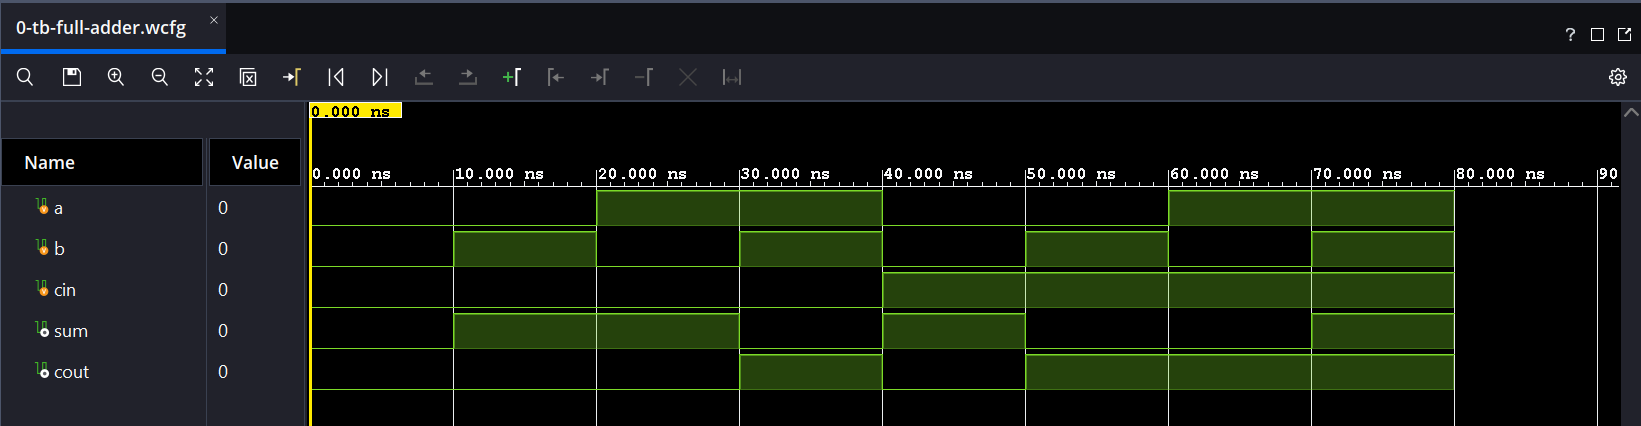
\includegraphics[width=\textwidth]{images/0-tb-full-adder.png}
\caption{一位全加器真值表仿真}
\end{figure}
波形以10 ns间隔遍历八种输入。三个输入全0时和与进位均为0；只有一个输入为1时和为1、进位为0；两个输入为1时和为0、进位为1；三个输入全1时两位输出均为1。八行结果均通过自动比较。

\subsection{多位加法器和先行进位加法器}
\begin{figure}[H]
\centering
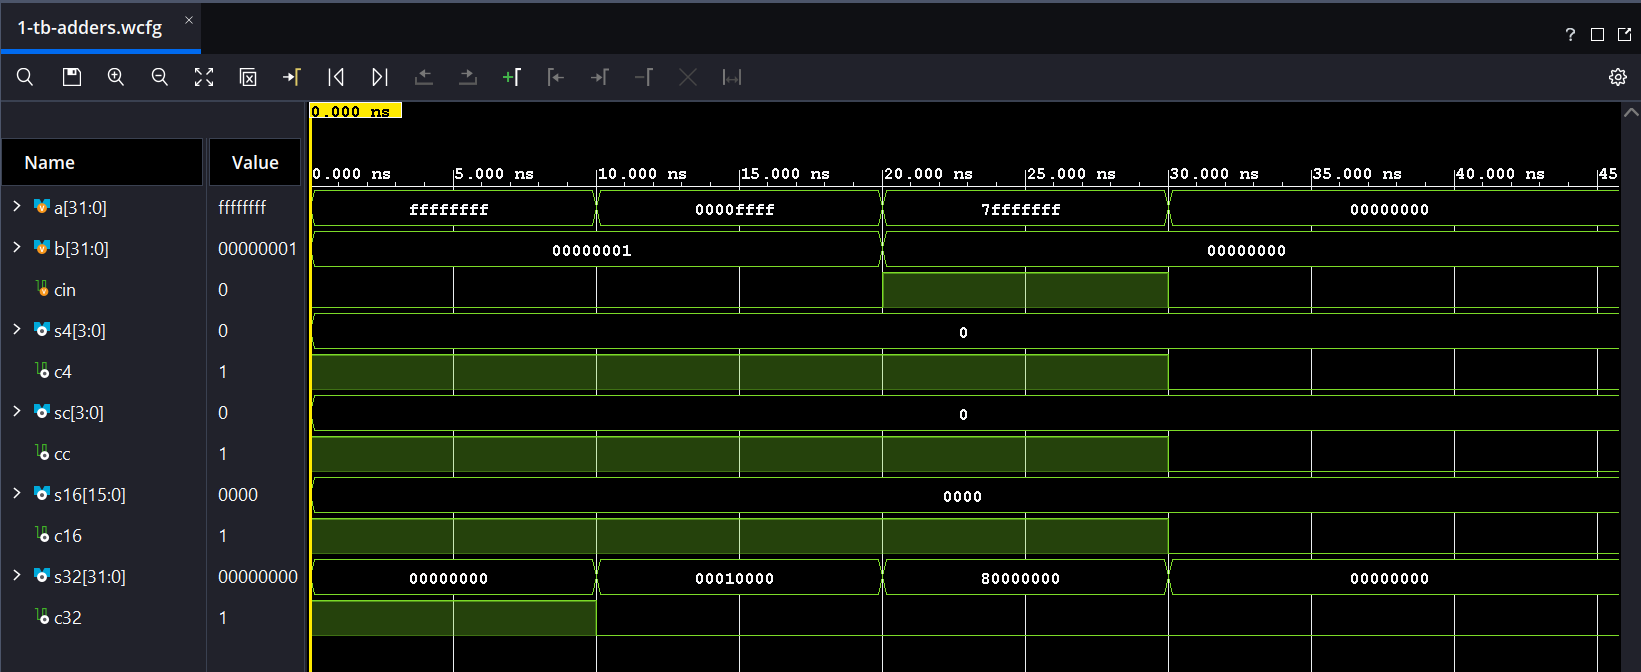
\includegraphics[width=\textwidth]{images/1-tb-adders.png}
\caption{多位加法器和先行进位加法器}
\end{figure}
前四组激励分别检查FFFFFFFF加1、0000FFFF加1、7FFFFFFF加进位1及全零情况。第一组32位和为0且最高进位置1，第二组16位和为0且16位进位置1，第三组32位结果为80000000。4位逐位进位和先行进位输出在这些输入下相同。随后遍历全部512种4位输入与进位组合，并对4、16、32位结果执行1000组固定种子随机检查，全部通过。

\subsection{八种操作的选择及两种实现对比}
\begin{figure}[H]
\centering
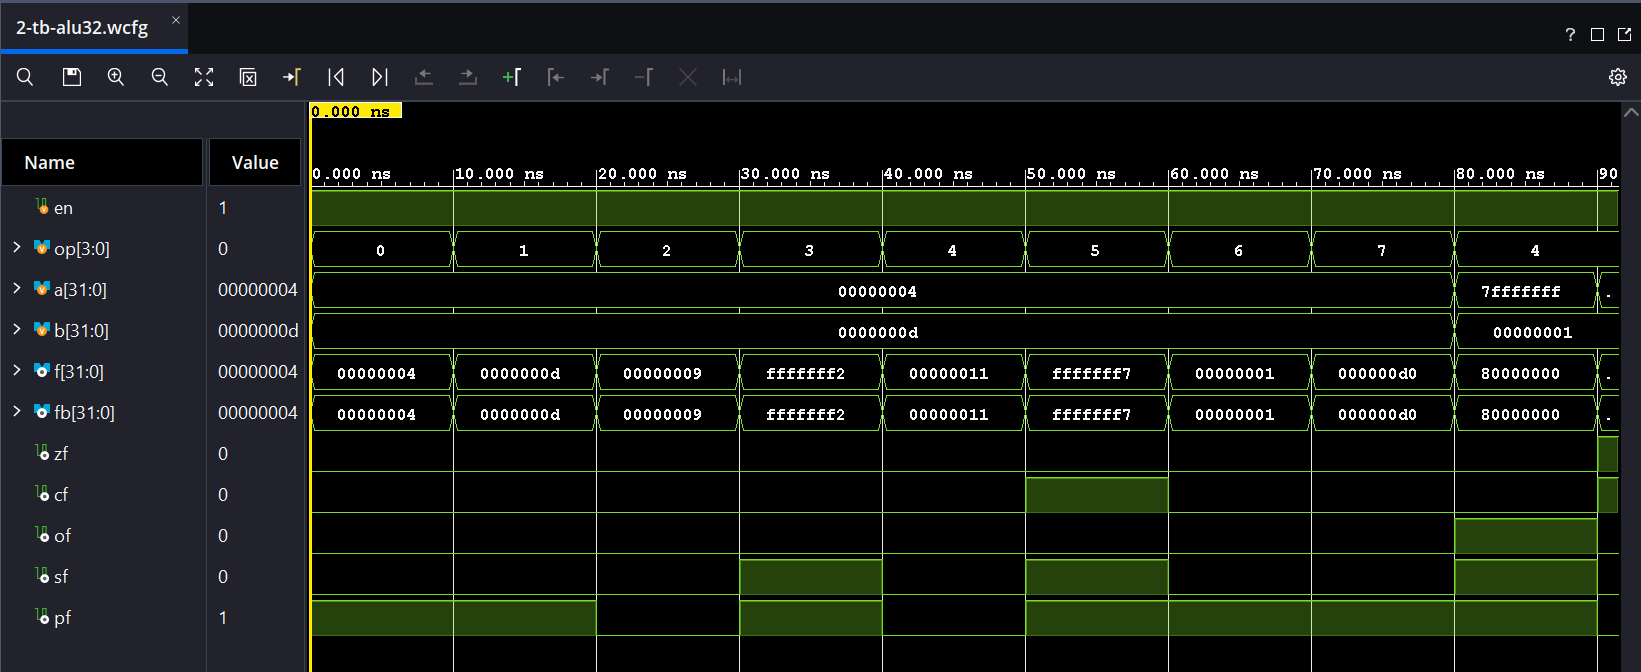
\includegraphics[width=\textwidth]{images/2-tb-alu32.png}
\caption{八种操作的选择及两种实现对比}
\end{figure}
A固定为4、B固定为13，操作码从0到7依次变化。十六进制结果依次为00000004、0000000D、00000009、FFFFFFF2、00000011、FFFFFFF7、00000001、000000D0。其中减法4减13得到负九的补码，比较4小于13输出1，左移将13左移4位得到208。行为结果f与共享总线结果fb一致。

\subsection{进位、借位与有符号溢出的边界}
\begin{figure}[H]
\centering
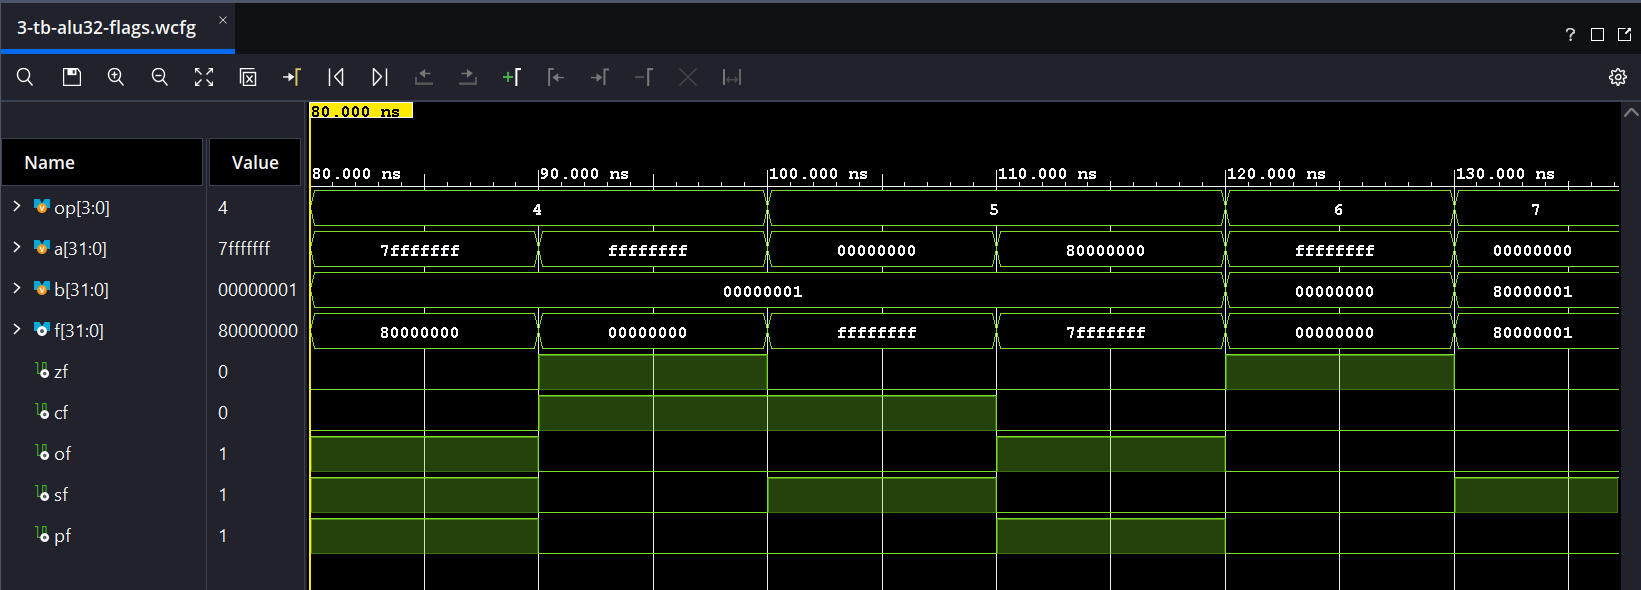
\includegraphics[width=\textwidth]{images/3-tb-alu32-flags.png}
\caption{进位、借位与有符号溢出的边界}
\end{figure}
80--90 ns计算7FFFFFFF加1，得到80000000，OF置1而CF为0；90--100 ns计算FFFFFFFF加1，结果为0，CF与ZF置1而OF为0。100--110 ns计算0减1，结果FFFFFFFF，借位CF置1；110--120 ns计算80000000减1，得到7FFFFFFF，有符号溢出OF置1而无符号借位为0。120--130 ns比较FFFFFFFF与0，输出0，说明SLT采用无符号语义。

\subsection{移位边界、关闭使能和保留编码}
\begin{figure}[H]
\centering
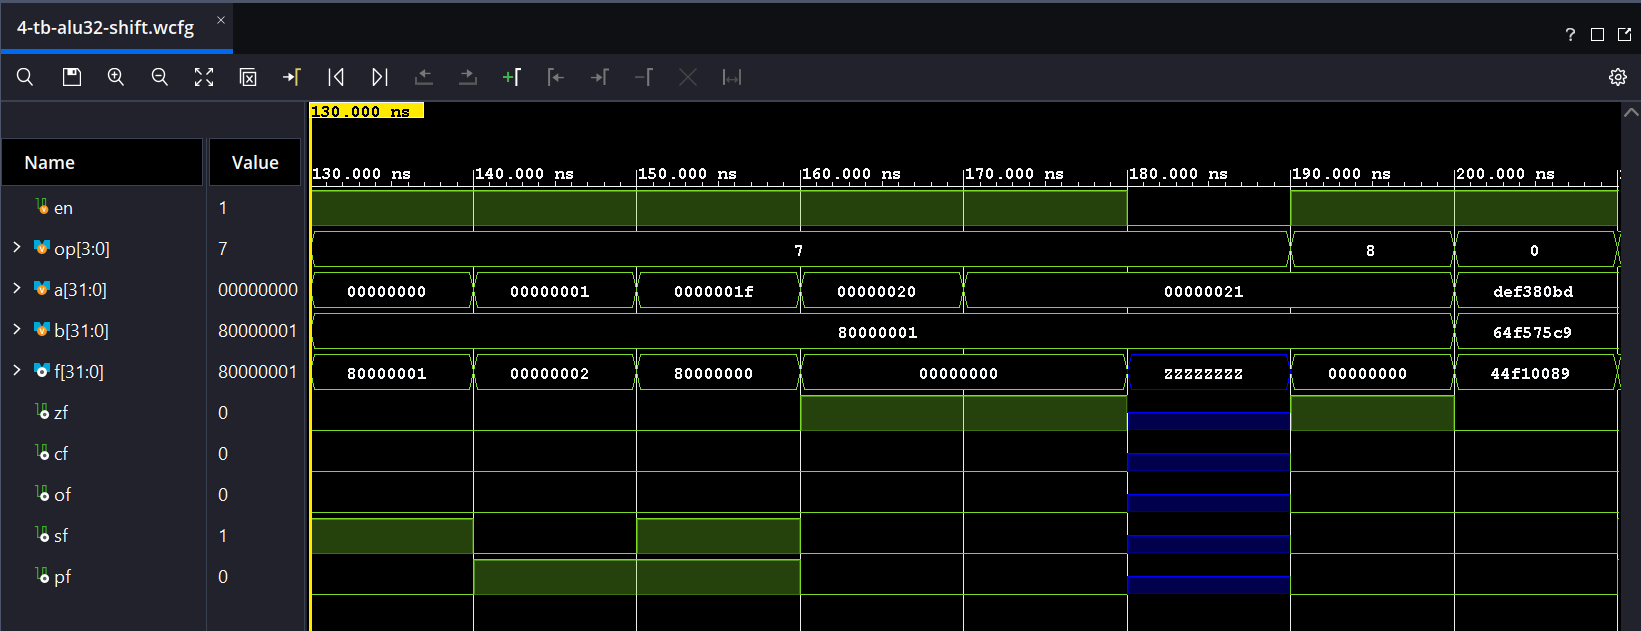
\includegraphics[width=\textwidth]{images/4-tb-alu32-shift.png}
\caption{移位边界、关闭使能和保留编码}
\end{figure}
B固定为80000001，移位量依次取0、1、31、32、33，结果分别为80000001、00000002、80000000、00000000、00000000。移位32位以上时结果清零，验证完整移位量的语义。180--190 ns关闭使能，结果和标志均为高阻态；190--200 ns恢复使能并选择保留编码8，结果为0，ZF置1，其余标志为0。

\subsection{共享总线的独热片选与输出释放}
\begin{figure}[H]
\centering
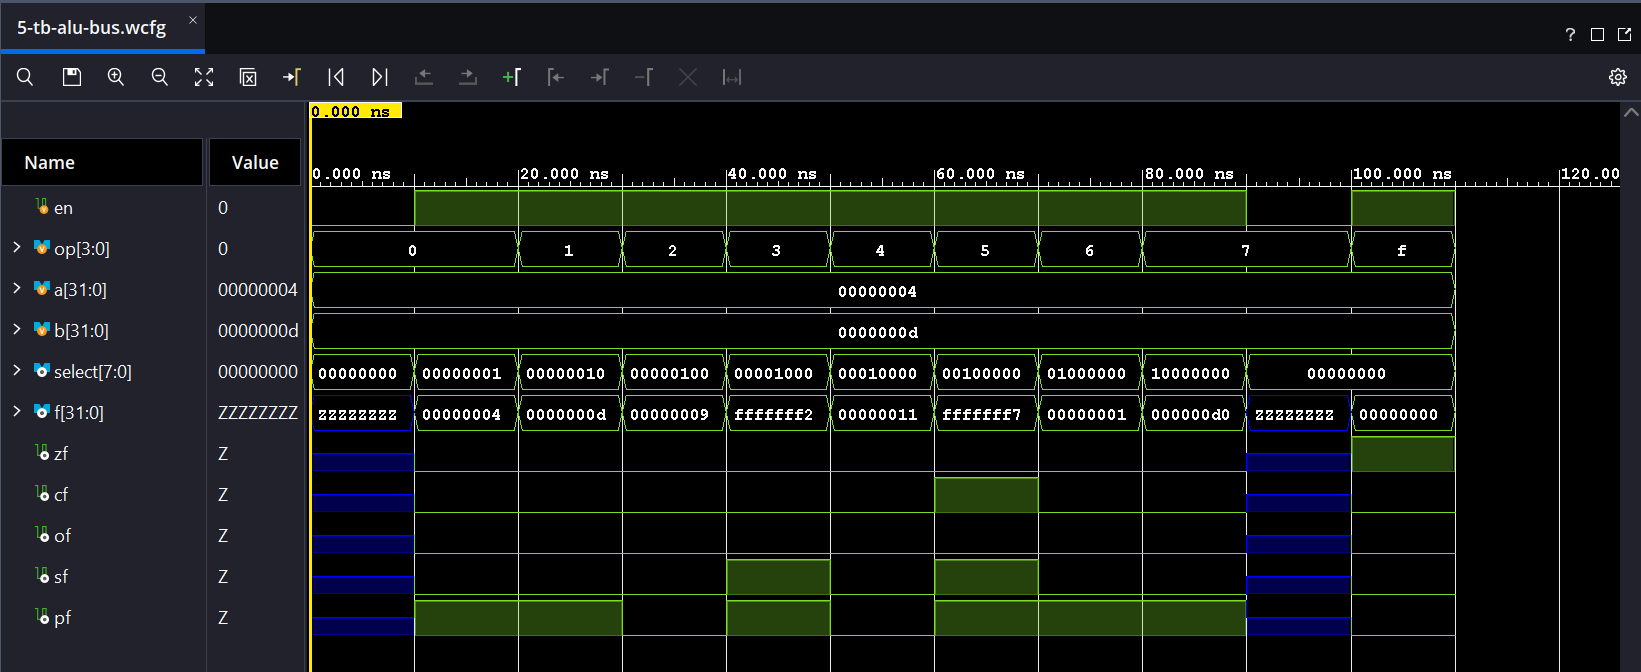
\includegraphics[width=\textwidth]{images/5-tb-alu-bus.png}
\caption{共享总线的独热片选与输出释放}
\end{figure}
0--10 ns使能无效，总线为高阻态。10--90 ns依次选中八个功能，select从00000001移动到10000000，始终只有一位置1，各段结果与行为版本相同。90--100 ns再次关闭使能，总线及标志释放；100--110 ns选择保留编码15，正常功能片选均为0，专门的保留编码分支驱动结果0。自动检查验证了译码、重复使能和高阻输出。

\subsection{自动检查汇总}
ALU测试在20组定向激励后，使用2000对固定种子随机操作数，逐对检查全部16种操作码，共32000组随机操作码检查。每组同时比较32位结果和五个标志，并检查行为实现与共享总线实现一致。实际运行摘要如下：
\begin{lstlisting}[language={}]
Vivado XSim 2026.1 - Lab 3 self-checking behavioral simulations
Combinational circuits; stimulus interval 10 ns.
PASS tb_adders: 4 directed + 512 exhaustive + 1000 random; widths 4/16/32 and CLA4
PASS tb_alu_bus: disable/re-enable, 8 one-hot selections, reserved opcode
PASS tb_alu32: 20 directed + 32000 random opcode checks; all results/flags and bus equivalence
PASS tb_full_adder: all 8 truth-table rows
ALL 4 TESTBENCHES PASSED
\end{lstlisting}
一位全加器覆盖全部真值表，多位加法器覆盖4位穷举与多位随机数据，ALU覆盖正常功能、保留编码、使能和数值边界。所有通过信息均在对应测试完成后打印，四个测试平台均正常结束。

\section{总结}
本实验完成一位全加器、参数化逐位进位加法器、层次化16位加法器和4位先行进位加法器，并完成八功能32位ALU及片选控制的共享总线版本。四个测试平台全部通过，波形与参考结果一致。

加法器级联说明了如何从基本逻辑门组合出多位算术电路，先行进位表达式展示了通过展开进位方程改变结构的方法。ALU将多个运算结果汇聚到一个输出，操作码选择可以用组合case描述，也可以通过功能译码和互斥片选控制总线。

标志位必须结合运算含义定义。无符号进位、借位与有符号溢出有不同判据；移位量是否截断会影响32及以上位移的结果；奇偶标志还需要明确统计范围和奇偶方向。本实现将这些规则写入接口说明，并在测试平台中用边界值和独立参考算法检查，使结果可重复验证。

\clearpage
\section*{附录：完整源代码和运行方法}
\addcontentsline{toc}{section}{附录：完整源代码和运行方法}
下面直接嵌入实际仿真使用的设计文件和测试平台，便于将报告与图像一起复制后阅读。
\subsection*{设计模块}
\subsubsection*{\texttt{adders.v}}
\begin{lstlisting}
`timescale 1ns / 1ps
module ripple_adder #(parameter WIDTH=32)(input wire [WIDTH-1:0] a,b,
 input wire cin, output wire [WIDTH-1:0] sum, output wire cout);
 wire [WIDTH:0] c;
 assign c[0]=cin; assign cout=c[WIDTH];
 genvar i;
 generate for(i=0;i<WIDTH;i=i+1) begin:g
  full_adder u(a[i],b[i],c[i],sum[i],c[i+1]);
 end endgenerate
endmodule

module cla4(input wire [3:0] a,b, input wire cin,
 output wire [3:0] sum, output wire cout);
 wire [3:0] p,g; wire [4:0] c;
 assign p=a^b; assign g=a&b; assign c[0]=cin;
 assign c[1]=g[0]|(p[0]&cin);
 assign c[2]=g[1]|(p[1]&g[0])|(p[1]&p[0]&cin);
 assign c[3]=g[2]|(p[2]&g[1])|(p[2]&p[1]&g[0])|(p[2]&p[1]&p[0]&cin);
 assign c[4]=g[3]|(p[3]&g[2])|(p[3]&p[2]&g[1])|
             (p[3]&p[2]&p[1]&g[0])|(p[3]&p[2]&p[1]&p[0]&cin);
 assign sum=p^c[3:0]; assign cout=c[4];
endmodule

// Four 4-bit blocks form a 16-bit hierarchical adder.
module adder16(input wire [15:0] a,b, input wire cin,
 output wire [15:0] sum, output wire cout);
 wire [4:0] c; assign c[0]=cin; assign cout=c[4];
 genvar k;
 generate for(k=0;k<4;k=k+1) begin:g
  ripple_adder #(.WIDTH(4)) u(a[k*4+:4],b[k*4+:4],c[k],sum[k*4+:4],c[k+1]);
 end endgenerate
endmodule
\end{lstlisting}
参数化模块逐位级联，16位模块按4位分组，CLA4直接展开全部进位。

\subsubsection*{\texttt{alu32.v}}
\begin{lstlisting}
`timescale 1ns / 1ps
module alu_flags(input wire [3:0] op,input wire [31:0] a,b,f,
 input wire cf_in,output wire zf,cf,of,sf,pf);
 assign zf=(f==0); assign sf=f[31]; assign pf=^f;
 assign cf=((op==4)||(op==5)) ? cf_in:1'b0;
 assign of=(op==4) ? ((~(a[31]^b[31]))&(f[31]^a[31])):
           (op==5) ? ((a[31]^b[31])&(f[31]^a[31])):1'b0;
endmodule

module alu32(input wire en,input wire [3:0] op,input wire [31:0] a,b,
 output wire [31:0] f,output wire zf,cf,of,sf,pf);
 reg [31:0] result; reg [32:0] extended;
 wire z,c,o,s,p;
 always @(*) begin
  result=0; extended=0;
  case(op)
   0: result=a&b;
   1: result=a|b;
   2: result=a^b;
   3: result=~(a|b);
   4: begin extended={1'b0,a}+{1'b0,b}; result=extended[31:0]; end
   5: begin extended={1'b0,a}-{1'b0,b}; result=extended[31:0]; end
   6: result=(a<b)?32'd1:32'd0;
   7: result=b<<a;
   default: result=0;
  endcase
 end
 alu_flags flags(op,a,b,result,extended[32],z,c,o,s,p);
 assign f=en?result:32'bz;
 assign {zf,cf,of,sf,pf}=en?{z,c,o,s,p}:5'bzzzzz;
endmodule
\end{lstlisting}
默认赋值和case产生确定结果，统一计算标志，并通过使能控制结果及标志的高阻输出。

\subsubsection*{\texttt{alu\_bus.v}}
\begin{lstlisting}
`timescale 1ns / 1ps
// Each operation drives the shared bus only when selected.
module alu_bus(input wire en,input wire [3:0] op,input wire [31:0] a,b,
 output wire [31:0] f,output wire zf,cf,of,sf,pf);
 wire [7:0] select;
 wire [31:0] value[0:7];
 wire add_cout,sub_cout;
 wire [31:0] bus_data;
 assign value[0]=a&b; assign value[1]=a|b;
 assign value[2]=a^b; assign value[3]=~(a|b);
 ripple_adder add(a,b,1'b0,value[4],add_cout);
 ripple_adder sub(a,~b,1'b1,value[5],sub_cout);
 assign value[6]=(a<b)?32'd1:32'd0;
 assign value[7]=b<<a;
 genvar i;
 generate for(i=0;i<8;i=i+1) begin:g
  assign select[i]=en&&(op==i);
  assign bus_data=select[i]?value[i]:32'bz;
 end endgenerate
 // Reserved operations have a defined zero result while enabled.
 assign bus_data=(en&&op[3])?32'b0:32'bz;
 assign f=bus_data;
 wire carry=(op==4)?add_cout:(op==5)?~sub_cout:1'b0;
 wire z,c,o,s,p;
 alu_flags flags(op,a,b,bus_data,carry,z,c,o,s,p);
 assign {zf,cf,of,sf,pf}=en?{z,c,o,s,p}:5'bzzzzz;
endmodule
\end{lstlisting}
八个独立驱动分支共享总线，结构化加法器完成加减法，减法最高进位取反形成借位。

\subsubsection*{\texttt{full\_adder.v}}
\begin{lstlisting}
`timescale 1ns / 1ps
module full_adder(input wire a,b,cin, output wire sum,cout);
 assign sum=a^b^cin;
 assign cout=(a&b)|(a&cin)|(b&cin);
endmodule
\end{lstlisting}
按真值表的异或和多数逻辑产生两位算术结果。

\subsection*{自检查测试平台}
\subsubsection*{\texttt{tb\_adders.v}}
\begin{lstlisting}
`timescale 1ns / 1ps
module tb_adders;
 reg [31:0] a,b; reg cin;
 wire [31:0] s32; wire c32;
 wire [15:0] s16; wire c16;
 wire [3:0] s4,sc; wire c4,cc;
 reg [32:0] expected; integer i,j,k,seed=12345;
 ripple_adder u32(a,b,cin,s32,c32);
 adder16 u16(a[15:0],b[15:0],cin,s16,c16);
 ripple_adder #(.WIDTH(4)) u4(a[3:0],b[3:0],cin,s4,c4);
 cla4 uc(a[3:0],b[3:0],cin,sc,cc);
 task check;
 begin
  #10; expected={1'b0,a}+{1'b0,b}+cin;
  if({c32,s32}!==expected) $fatal(1,"32-bit adder");
  if({c16,s16}!==({1'b0,a[15:0]}+{1'b0,b[15:0]}+cin)) $fatal(1,"16-bit adder");
  if({c4,s4}!==({1'b0,a[3:0]}+{1'b0,b[3:0]}+cin)) $fatal(1,"4-bit adder");
  if({cc,sc}!=={c4,s4}) $fatal(1,"CLA mismatch");
 end endtask
 initial begin
  a=32'hffffffff;b=1;cin=0;check;
  a=32'h0000ffff;b=1;cin=0;check;
  a=32'h7fffffff;b=0;cin=1;check;
  a=0;b=0;cin=0;check;
  for(i=0;i<16;i=i+1) for(j=0;j<16;j=j+1) for(k=0;k<2;k=k+1) begin
   a=i;b=j;cin=k;check;
  end
  for(i=0;i<1000;i=i+1) begin a=$random(seed);b=$random(seed);cin=$random(seed);check;end
  $display("PASS tb_adders: 4 directed + 512 exhaustive + 1000 random; widths 4/16/32 and CLA4");$finish;
 end
endmodule
\end{lstlisting}
四个实例接受相同输入，在定向、穷举及随机激励下与扩展算术结果比较。

\subsubsection*{\texttt{tb\_alu32.v}}
\begin{lstlisting}
`timescale 1ns / 1ps
module tb_alu32;
 reg en;reg [3:0] op;reg [31:0] a,b;
 wire [31:0] f,fb;wire zf,cf,of,sf,pf,zb,cb,ob,sb,pb;
 reg [31:0] expected;reg ec,eo,ep;reg [32:0] wide;
 reg signed [63:0] signed_result;
 integer i,j,k,seed=271799;
 alu32 dut(en,op,a,b,f,zf,cf,of,sf,pf);
 alu_bus bus_dut(en,op,a,b,fb,zb,cb,ob,sb,pb);
 task check;
 begin
  #10;
  if(!en) begin
   if({f,zf,cf,of,sf,pf}!==37'bz || {fb,zb,cb,ob,sb,pb}!==37'bz) $fatal(1,"disable failed");
  end else begin
   expected=0;ec=0;eo=0;wide=0;signed_result=0;
   case(op)
    0: expected=a&b; 1: expected=a|b; 2: expected=a^b; 3:expected=~(a|b);
    4:begin wide={1'b0,a}+{1'b0,b};expected=wide[31:0];ec=wide[32];
      signed_result=$signed({{32{a[31]}},a})+$signed({{32{b[31]}},b});end
    5:begin expected=a-b;ec=(a<b);
      signed_result=$signed({{32{a[31]}},a})-$signed({{32{b[31]}},b});end
    6:expected=(a<b);7:expected=(a>=32)?0:(b<<a);
   endcase
   if(op==4||op==5) eo=(signed_result>64'sd2147483647)||(signed_result< -64'sd2147483648);
   ep=0;for(k=0;k<32;k=k+1) ep=ep^expected[k];
   if({f,zf,cf,of,sf,pf}!=={expected,(expected==0),ec,eo,expected[31],ep})
    $fatal(1,"ALU failed op=%h a=%h b=%h f=%h",op,a,b,f);
   if({fb,zb,cb,ob,sb,pb}!=={f,zf,cf,of,sf,pf}) $fatal(1,"bus mismatch");
  end
 end endtask
 initial begin
  en=1;a=4;b=13;
  for(j=0;j<8;j=j+1)begin op=j;check;end
  op=4;a=32'h7fffffff;b=1;check;
  a=32'hffffffff;b=1;check;
  op=5;a=0;b=1;check;
  a=32'h80000000;b=1;check;
  op=6;a=32'hffffffff;b=0;check;
  op=7;b=32'h80000001;
  a=0;check;a=1;check;a=31;check;a=32;check;a=33;check;
  en=0;check;en=1;op=8;check;
  for(i=0;i<2000;i=i+1) begin
   a=$random(seed);b=$random(seed);
   for(j=0;j<16;j=j+1)begin op=j;check;end
  end
  $display("PASS tb_alu32: 20 directed + 32000 random opcode checks; all results/flags and bus equivalence");$finish;
 end
endmodule
\end{lstlisting}
独立计算结果、借位、溢出和奇偶标志，同时比较两种ALU实现。固定随机种子保证运行可重复。

\subsubsection*{\texttt{tb\_alu\_bus.v}}
\begin{lstlisting}
`timescale 1ns / 1ps
module tb_alu_bus;
 reg en;reg [3:0] op;reg [31:0] a,b;
 wire [31:0] f;wire zf,cf,of,sf,pf;integer i;
 alu_bus dut(en,op,a,b,f,zf,cf,of,sf,pf);
 initial begin
  a=4;b=13;en=0;op=0;#10;
  if(f!==32'bz) $fatal(1,"bus not released");
  en=1;
  for(i=0;i<8;i=i+1)begin op=i;#10;
   if(dut.select!==(8'b1<<i)) $fatal(1,"decoder not one-hot");
  end
  en=0;#10;if({f,zf,cf,of,sf,pf}!==37'bz) $fatal(1,"disable");
  en=1;op=15;#10;if(f!==0||dut.select!==0) $fatal(1,"reserved opcode");
  $display("PASS tb_alu_bus: disable/re-enable, 8 one-hot selections, reserved opcode");$finish;
 end
endmodule
\end{lstlisting}
直接检查内部独热片选、关闭使能后的总线释放和保留编码输出。

\subsubsection*{\texttt{tb\_full\_adder.v}}
\begin{lstlisting}
`timescale 1ns / 1ps
module tb_full_adder;
 reg a,b,cin; wire sum,cout; integer i;
 full_adder dut(a,b,cin,sum,cout);
 initial begin
  for(i=0;i<8;i=i+1) begin
   {cin,a,b}=i; #10;
   if({cout,sum} !== ( {1'b0,a}+{1'b0,b}+cin)) $fatal(1,"full adder failed");
  end
  $display("PASS tb_full_adder: all 8 truth-table rows"); $finish;
 end
endmodule
\end{lstlisting}
穷举全部八种输入，并检查完整的和与进位。

\subsection*{运行方法}
在Vivado Tcl控制台中执行：
\begin{lstlisting}[language={}]
source D:/Local/Github/XJTU-Labs/Computer-Organization/lab-3/setup_lab3.tcl
lab3_sim tb_alu32
\end{lstlisting}
第一条命令注册设计源文件和仿真源文件，第二条选择ALU测试顶层并运行到结束。将顶层替换为其他测试平台可查看相应任务。

在实验目录的PowerShell中执行以下命令，可以统一完成四个平台的编译、展开和仿真：
\begin{lstlisting}[language={}]
.\run_all.ps1
\end{lstlisting}
脚本遇到编译失败、展开失败或没有通过信息时会停止，全部测试成功后才生成完整通过汇总。

查看已保存的结果可执行：
\begin{lstlisting}[language={}]
source D:/Local/Github/XJTU-Labs/Computer-Organization/lab-3/view_results.tcl
lab3_view 3-tb-alu32-flags
\end{lstlisting}
这两条命令直接打开已记录的波形数据库，并载入标志位截图所用的信号和时间区间，无需重新产生输入激励。
\end{document}
